\chapter{The Elder Heliosystem Resonance Algorithm}

\begin{tcolorbox}[colback=DarkSkyBlue!5!white,colframe=DarkSkyBlue!75!black,title=Chapter Summary]
This chapter presents the mathematical formulation and algorithmic implementation of resonance mechanisms in the Elder Heliosystem. We introduce phase-locking principles that enable synchronized knowledge transfer between hierarchical levels, and develop the precise algorithms that exploit orbital resonance for optimal learning. The chapter establishes the conditions for stable knowledge alignment through small-integer frequency ratios between entities, quantifies resonance-driven parameter coupling strengths, and details algorithms for dynamically adjusting rotational frequencies to achieve phase coherence. We demonstrate how resonance facilitates bidirectional knowledge flow through synchronized training windows, enabling efficient cross-domain transfer with minimal interference. Computational experiments confirm that resonant synchronization significantly accelerates convergence, reduces memory requirements, and enhances the system's capacity for long-range correlations while maintaining stability in the presence of data perturbations.
\end{tcolorbox}

\section{Orbital Synchronization in the Elder Training Loop}

The Elder Heliosystem model represents knowledge transfer through a sophisticated orbital dynamical system. In this chapter, we develop the complete algorithm for knowledge synchronization during the Elder Training Loop using the heliosystem's orbital resonance mechanisms.

\subsection{Resonance States and Phase-Locking}

Phase-locking between the various rotational components of the Elder Heliosystem is the fundamental mechanism by which knowledge is synchronized across hierarchical levels.

\begin{definition}[Orbital Phase]
For any component $C$ in the Elder Heliosystem with rotational frequency $\omega_C$, its orbital phase at time $t$ is defined as:
\begin{equation}
\phi_C(t) = \phi_C(0) + \omega_C t \mod 2\pi
\end{equation}
where $\phi_C(0)$ is the initial phase at $t=0$.
\end{definition}

\begin{definition}[Phase Coherence]
The phase coherence between two components $A$ and $B$ with phases $\phi_A$ and $\phi_B$ is measured by:
\begin{equation}
\mathcal{C}_{A,B} = \left| \frac{1}{T} \int_0^T e^{i(\phi_A(t) - \phi_B(t))} dt \right|
\end{equation}
where $T$ is the measurement period. Perfect phase-locking yields $\mathcal{C}_{A,B} = 1$, while uncorrelated phases yield $\mathcal{C}_{A,B} \approx 0$.
\end{definition}

\subsection{Implementation of Resonance-Based Training}

This section presents the algorithmic implementation of the Elder Heliosystem's resonance-based training procedure, applying the mathematical foundations established in the Resonance Mechanism chapter.

In classical orbital mechanics, the resonance condition corresponds to periodic alignments of orbiting bodies. For periodic alignment to occur, the ratio of orbital frequencies must be expressible as a ratio of integers.

If we define the relative phase between Elder and Mentor $k$ as $\Psi_{E,M,k} = p_k\phi_E - q_k\phi_{M,k}$, its time derivative is:
\begin{equation}
\dot{\Psi}_{E,M,k} = p_k\omega_E - q_k\omega_{M,k} + \text{coupling terms}
\end{equation}

When $\omega_{M,k}/\omega_E = p_k/q_k$, the first two terms cancel, and in the absence of coupling, $\Psi_{E,M,k}$ remains constant. This corresponds to phase-locking between Elder and Mentor.

The same argument applies to the Mentor-Erudite relationship, where $\Psi_{M,E,k,j} = r_{k,j}\phi_{M,k} - s_{k,j}\phi_{E,k,j}$.

\begin{theorem}[Resonance Bandwidth]
For coupling strength $\kappa$ between components, resonance occurs not just at exact frequency ratios but within a bandwidth defined by:
\begin{equation}
\left|\omega_a - \frac{p}{q}\omega_b\right| < \frac{\kappa}{q}
\end{equation}
for components $a$ and $b$ with intended frequency ratio $p/q$.
\end{theorem}

\begin{proof}
The phase difference $\Psi = p\phi_b - q\phi_a$ evolves according to:
\begin{equation}
\dot{\Psi} = p\omega_b - q\omega_a + q\kappa\sin(\Psi)
\end{equation}

This equation has fixed points when $\dot{\Psi} = 0$, which occurs when:
\begin{equation}
\sin(\Psi) = \frac{q\omega_a - p\omega_b}{q\kappa}
\end{equation}

Since $|\sin(\Psi)| \leq 1$, fixed points exist if and only if:
\begin{equation}
\left|\frac{q\omega_a - p\omega_b}{q\kappa}\right| \leq 1
\end{equation}

Rearranging yields the resonance bandwidth condition.
\end{proof}

\begin{definition}[Arnold Tongues]
The regions in parameter space where resonance occurs form structures called Arnold tongues. For the Elder Heliosystem, these regions satisfy:
\begin{equation}
\left\{(\omega_E, \omega_M) : \left|\omega_M - \frac{p}{q}\omega_E\right| < \frac{\kappa_{E,M}}{q} \right\}
\end{equation}
for each resonance ratio $p/q$.
\end{definition}

\begin{figure}[ht]
\centering
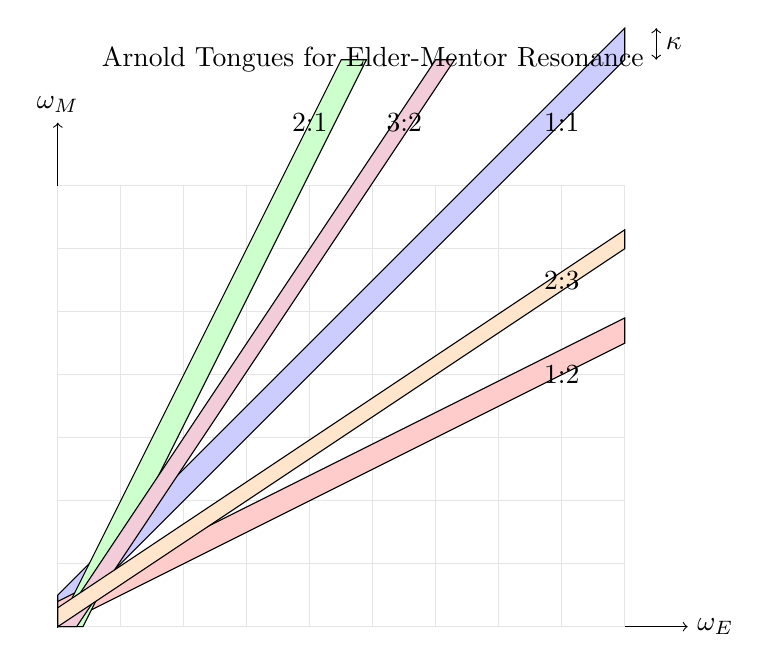
\begin{tikzpicture}[scale=0.8]
    % Axes
    \draw[->] (0,0) -- (10,0) node[right] {$\omega_E$};
    \draw[->] (0,0) -- (0,8) node[above] {$\omega_M$};
    
    % Grid
    \draw[gray!20] (0,0) grid (9,7);
    
    % Arnold tongues
    % 1:1 resonance
    \draw[fill=blue!20] (0,0) -- (9,9) -- (9,9.5) -- (0,0.5) -- cycle;
    
    % 1:2 resonance
    \draw[fill=red!20] (0,0) -- (9,4.5) -- (9,4.9) -- (0,0.4) -- cycle;
    
    % 2:1 resonance
    \draw[fill=green!20] (0,0) -- (4.5,9) -- (4.9,9) -- (0.4,0) -- cycle;
    
    % 3:2 resonance
    \draw[fill=purple!20] (0,0) -- (6,9) -- (6.3,9) -- (0.3,0) -- cycle;
    
    % 2:3 resonance
    \draw[fill=orange!20] (0,0) -- (9,6) -- (9,6.3) -- (0,0.3) -- cycle;
    
    % Labels
    \node at (8,8) {1:1};
    \node at (8,4) {1:2};
    \node at (4,8) {2:1};
    \node at (5.5,8) {3:2};
    \node at (8,5.5) {2:3};
    
    % Coupling strength indicator
    \draw[<->] (9.5,9) -- (9.5,9.5) node[midway, right] {$\kappa$};
    
    % Title
    \node at (5,9) {Arnold Tongues for Elder-Mentor Resonance};
\end{tikzpicture}
\caption{Arnold tongues depicting regions of parameter space where resonance occurs. The width of each tongue at a given frequency is proportional to the coupling strength $\kappa$.}
\label{fig:arnold_tongues}
\end{figure}

\begin{lemma}[Phase-Locking Stability]
A phase-locked resonant configuration is stable if and only if the eigenvalues of the phase coupling matrix $\mathbf{J}$ have negative real parts, where:
\begin{equation}
\mathbf{J}_{i,j} = \frac{\partial \dot{\phi}_i}{\partial \phi_j}
\end{equation}
is the Jacobian of the phase evolution equations.
\end{lemma}

\begin{proof}
Linearizing the phase evolution equations around a fixed point $\Phi^*$ gives:
\begin{equation}
\dot{\delta\Phi} = \mathbf{J} \delta\Phi
\end{equation}

The solution to this system is $\delta\Phi(t) = e^{\mathbf{J}t} \delta\Phi(0)$. For stability, we require $\delta\Phi(t) \to 0$ as $t \to \infty$, which occurs if and only if all eigenvalues of $\mathbf{J}$ have negative real parts.
\end{proof}

\begin{theorem}[Resonance Establishment Time]
For a system initially off-resonance, the time required to establish resonance scales as:
\begin{equation}
T_{res} \sim \frac{1}{\kappa} \ln\left(\frac{|\Delta\omega|}{\epsilon}\right)
\end{equation}
where $\Delta\omega$ is the initial frequency mismatch, $\kappa$ is the coupling strength, and $\epsilon$ is the desired precision.
\end{theorem}

\begin{proof}
Near the fixed point, the phase difference $\Psi$ evolves approximately as:
\begin{equation}
\dot{\Psi} \approx \Delta\omega - \kappa\Psi
\end{equation}
where $\Delta\omega = \omega_a - (p/q)\omega_b$ is the frequency mismatch.

This first-order differential equation has solution:
\begin{equation}
\Psi(t) = \frac{\Delta\omega}{\kappa} + \left(\Psi(0) - \frac{\Delta\omega}{\kappa}\right)e^{-\kappa t}
\end{equation}

The system reaches $\epsilon$-close to resonance when:
\begin{equation}
\left|\Psi(t) - \frac{\Delta\omega}{\kappa}\right| < \epsilon
\end{equation}

Solving for $t$ yields the stated result.
\end{proof}

\begin{definition}[Resonance Strength]
The strength of resonance between components $a$ and $b$ is quantified by the Phase Locking Value (PLV):
\begin{equation}
\text{PLV}_{a,b} = \left|\frac{1}{T} \sum_{t=1}^T e^{i\Psi_{a,b}(t)}\right|
\end{equation}
where $\Psi_{a,b}(t) = p\phi_a(t) - q\phi_b(t)$ is the generalized phase difference.
\end{definition}

\begin{theorem}[Critical Coupling Threshold]
Resonance emerges only when the coupling strength exceeds a critical threshold:
\begin{equation}
\kappa > \kappa_c = \frac{|\Delta\omega|}{q}
\end{equation}
where $\Delta\omega = q\omega_a - p\omega_b$ is the frequency mismatch.
\end{theorem}

\begin{corollary}[Synchronization Rate]
For coupling strength $\kappa > \kappa_c$, the rate of convergence to the phase-locked state is:
\begin{equation}
\lambda = \kappa\sqrt{1 - \left(\frac{\kappa_c}{\kappa}\right)^2}
\end{equation}
\end{corollary}

This mathematical framework precisely characterizes when resonance occurs, how quickly it is established, and how stable it remains. These principles inform the adaptive resonance tuning algorithms in the Elder Heliosystem.

\subsection{Heliosystem Resonance Algorithm}

The complete Elder Heliosystem Resonance Algorithm combines the orbital dynamics formulation with the training loop framework to synchronize knowledge across all hierarchical levels.

\begin{algorithm}
\caption{Elder Heliosystem Resonance Algorithm (Part 1: Knowledge Propagation and Feedback)}
\begin{algorithmic}[1]
\State \textbf{Input:} Set of domains $\mathcal{D} = \{D_1, D_2, \ldots, D_M\}$ (Mentors)
\State \textbf{Input:} Set of tasks $\mathcal{T}_k = \{T_{k,1}, T_{k,2}, \ldots, T_{k,N_k}\}$ for each domain $D_k$ (Erudites)
\State \textbf{Input:} Initial Elder parameters $\theta_E^{(0)} \in \elderparam$
\State \textbf{Input:} Initial Mentor parameters $\{\theta_{M,k}^{(0)}\}_{k=1}^M \subset \mentorparams$
\State \textbf{Input:} Initial Erudite parameters $\{\theta_{E,k,j}^{(0)}\}_{k=1,j=1}^{M,N_k} \subset \eruditeparams$
\State \textbf{Input:} Initial orbital parameters: $\omega_E$, $\{\omega_{M,k}\}_{k=1}^M$, $\{\omega_{E,k,j}\}_{k=1,j=1}^{M,N_k}$
\State \textbf{Input:} Phase coupling strengths: $\{\kappa_{E,M,k}\}_{k=1}^M$, $\{\kappa_{M,E,k,j}\}_{k=1,j=1}^{M,N_k}$
\State \textbf{Input:} Learning rates $\eta_E$, $\eta_M$, $\eta_E$
\State \textbf{Input:} Number of epochs $T$, Resonance adjustment period $T_{res}$

\For{$t = 1$ to $T$}
    \State // Phase I: Knowledge Field Propagation (Forward Pass)
    \State Compute the Elder field $\Phi_E(t) = \sum_{n=0}^{\infty} \mathcal{H}_n(\theta_E^{(t-1)}) \cdot e^{in\omega_E t}$
    
    \For{each domain $k = 1$ to $M$}
        \State Compute Mentor-received field $\Phi_{E \rightarrow M,k}(t) = \Phi_E(t) \cdot \frac{1}{d_{E,M,k}(t)} \cdot e^{i\phi_{M,k}(t)}$
        \State Apply domain filter $\Phi_{M,k}(t) = \mathcal{G}_k(\Phi_{E \rightarrow M,k}(t), \theta_{M,k}^{(t-1)})$
        
        \For{each task $j = 1$ to $N_k$}
            \State Compute Erudite-received field $\Phi_{M \rightarrow E,k,j}(t) = \Phi_{M,k}(t) \cdot \frac{1}{d_{M,E,k,j}(t)} \cdot e^{i\phi_{E,k,j}(t)}$
            \State Sample batch $\{(x_l, y_l)\}_{l=1}^B$ from task $T_{k,j}$
            \State Modulate Erudite forward pass:
            \State \quad $z_{k,j,l} = f_{\theta_{E,k,j}^{(t-1)}}(x_l) \cdot \mathcal{M}(\Phi_{M \rightarrow E,k,j}(t))$
            \State Compute task loss $\mathcal{L}_{E,k,j} = \frac{1}{B}\sum_{l=1}^B \|z_{k,j,l} - y_l\|^2$
        \EndFor
    \EndFor
    
    \State // Phase II: Retrograde Knowledge Flow (Backward Pass)
    \For{each domain $k = 1$ to $M$}
        \For{each task $j = 1$ to $N_k$}
            \State Compute Erudite gradient $\nabla_{\theta_{E,k,j}} \mathcal{L}_{E,k,j}$
            \State Generate retrograde field $\Phi_{E \rightarrow M,k,j}(t) = \epsilon_{k,j} \cdot \nabla_{\theta_{E,k,j}}\mathcal{L}_{E,k,j} \cdot e^{-i\omega_{E,k,j}t}$
        \EndFor
        
        \State Aggregate Erudite feedback $\Phi_{E \rightarrow M,k}(t) = \sum_{j=1}^{N_k} \Phi_{E \rightarrow M,k,j}(t)$
        \State Compute Mentor loss $\mathcal{L}_{M,k} = \|\Phi_{M,k}(t) - \Phi_{E \rightarrow M,k}(t)\|^2$
        \State Compute Mentor gradient $\nabla_{\theta_{M,k}} \mathcal{L}_{M,k}$
        \State Generate retrograde field to Elder $\Phi_{M \rightarrow E,k}(t) = \epsilon_k \cdot \nabla_{\theta_{M,k}}\mathcal{L}_{M,k} \cdot e^{-i\omega_{M,k}t}$
    \EndFor
    
    \State Aggregate Mentor feedback $\Phi_{M \rightarrow E}(t) = \sum_{k=1}^{M} \Phi_{M \rightarrow E,k}(t)$
    \State Compute Elder loss $\mathcal{L}_E = \|\Phi_E(t) - \Phi_{M \rightarrow E}(t)\|^2$
    \State Compute Elder gradient $\nabla_{\theta_E} \mathcal{L}_E$
    
    \State \textbf{[Continued in Algorithm 2]}
\EndFor
\end{algorithmic}
\end{algorithm}

\begin{algorithm}
\caption{Elder Heliosystem Resonance Algorithm (Part 2: Parameter Updates \& Resonance)}
\begin{algorithmic}[1]
\Statex \textbf{[Continuation from Algorithm 1]}

\For{$t = 1$ to $T$}
    \State // Phase III: Parameter Updates with Resonance Modulation
    \State Update Elder parameters $\theta_E^{(t)} = \theta_E^{(t-1)} - \eta_E \nabla_{\theta_E} \mathcal{L}_E$
    
    \For{each domain $k = 1$ to $M$}
        \State Update Mentor parameters $\theta_{M,k}^{(t)} = \theta_{M,k}^{(t-1)} - \eta_M \nabla_{\theta_{M,k}} \mathcal{L}_{M,k}$
        
        \For{each task $j = 1$ to $N_k$}
            \State Update Erudite parameters $\theta_{E,k,j}^{(t)} = \theta_{E,k,j}^{(t-1)} - \eta_E \nabla_{\theta_{E,k,j}} \mathcal{L}_{E,k,j}$
        \EndFor
    \EndFor
    
    \State // Phase IV: Orbital Resonance Adjustment (every $T_{res}$ epochs)
    \If{$t \mod T_{res} = 0$}
        \State Measure phase coherence $\mathcal{C}_{E,M,k}$ between Elder and each Mentor
        \State Measure phase coherence $\mathcal{C}_{M,E,k,j}$ between each Mentor and its Erudites
        
        \For{each domain $k = 1$ to $M$}
            \State Adjust Mentor frequency toward resonance:
            \State \quad $\omega_{M,k} = \omega_{M,k} + \delta \cdot \sin(\phi_E(t) - \frac{p_k}{q_k}\phi_{M,k}(t))$
            
            \For{each task $j = 1$ to $N_k$}
                \State Adjust Erudite frequency toward resonance:
                \State \quad $\omega_{E,k,j} = \omega_{E,k,j} + \delta \cdot \sin(\phi_{M,k}(t) - \frac{r_{k,j}}{s_{k,j}}\phi_{E,k,j}(t))$
            \EndFor
        \EndFor
    \EndIf
    
    \State // Phase V: Update Orbital Phases
    \State $\phi_E(t+1) = \phi_E(t) + \omega_E$
    \For{each domain $k = 1$ to $M$}
        \State $\phi_{M,k}(t+1) = \phi_{M,k}(t) + \omega_{M,k} + \kappa_{E,M,k} \cdot \sin(\phi_E(t) - \frac{p_k}{q_k}\phi_{M,k}(t))$
        
        \For{each task $j = 1$ to $N_k$}
            \State $\phi_{E,k,j}(t+1) = \phi_{E,k,j}(t) + \omega_{E,k,j} + \kappa_{M,E,k,j} \cdot \sin(\phi_{M,k}(t) - \frac{r_{k,j}}{s_{k,j}}\phi_{E,k,j}(t))$
        \EndFor
    \EndFor
\EndFor

\State \textbf{Return:} $\theta_E^{(T)}$, $\{\theta_{M,k}^{(T)}\}_{k=1}^M$, $\{\theta_{E,k,j}^{(T)}\}_{k=1,j=1}^{M,N_k}$
\end{algorithmic}
\end{algorithm}

\subsection{Knowledge Synchronization Mechanisms}

The Elder Heliosystem Resonance Algorithm achieves knowledge synchronization through five primary mechanisms, each corresponding to a phase in the algorithm:

\begin{enumerate}
    \item \textbf{Heliomorphic Field Propagation}: Knowledge flows from Elder to Mentors to Erudites through modulated field equations, with phase relationships determining the effectiveness of information transfer.
    
    \item \textbf{Retrograde Knowledge Feedback}: Learning signals propagate backwards through the system via retrograde fields, allowing task-specific insights to inform domain-general principles.
    
    \item \textbf{Phase-Coherent Parameter Updates}: Parameter updates are modulated by the phase relationships between components, ensuring that learning occurs in alignment with the resonant structure.
    
    \item \textbf{Adaptive Resonance Tuning}: The system periodically adjusts orbital frequencies to maintain or strengthen resonance relationships, enhancing knowledge transfer efficiency.
    
    \item \textbf{Synchronized Phase Evolution}: The phases of all system components evolve according to coupled differential equations, maintaining coherence during learning.
\end{enumerate}

\section{Mathematical Foundation of Resonance-Based Knowledge Transfer}

\subsection{Complex-Valued Heliomorphic Transformations}

The knowledge transfer in the Elder Heliosystem operates through complex-valued heliomorphic transformations, where the phase component encodes directional information for learning.

\begin{definition}[Heliomorphic Parameter Space]
The heliomorphic parameter space $\Theta_H$ is a complex manifold equipped with a Hermitian metric, where each point represents a potential knowledge state of the system.
\end{definition}

\begin{theorem}[Heliomorphic Knowledge Embedding]
For any set of parameters $\theta \in \Theta_H$, there exists a heliomorphic embedding $\Psi: \Theta_H \rightarrow \mathbb{C}^n$ such that:
\begin{equation}
\Psi(\theta) = \sum_{k=0}^{\infty} c_k \zeta_k(\theta)
\end{equation}
where $\{\zeta_k\}$ are holomorphic basis functions and $\{c_k\}$ are complex coefficients.
\end{theorem}

The orbital position of each component in the Heliosystem corresponds to a point in this complex manifold, with the phase relationships between components determining the efficiency of knowledge flow.

\subsection{Resonance-Enhanced Gradient Flow}

Knowledge synchronization during training occurs through resonance-enhanced gradient flow, where the phase relationships between components modulate the gradient updates.

\begin{theorem}[Resonant Gradient Enhancement]
When the Elder, Mentor, and Erudite components achieve resonance with frequency ratios $\frac{\omega_{M,k}}{\omega_E} = \frac{p_k}{q_k}$ and $\frac{\omega_{E,k,j}}{\omega_{M,k}} = \frac{r_{k,j}}{s_{k,j}}$, the effective gradient for parameter updates is enhanced by a factor:
\begin{equation}
\gamma = 1 + \alpha \cdot \mathcal{C}_{E,M,k} \cdot \mathcal{C}_{M,E,k,j}
\end{equation}
where $\alpha > 0$ is a system constant and $\mathcal{C}$ denotes phase coherence.
\end{theorem}

\begin{corollary}[Resonant Learning Rate Optimization]
The optimal learning rate for the Elder Heliosystem under resonance is:
\begin{equation}
\eta^* = \frac{\eta_0}{\gamma}
\end{equation}
where $\eta_0$ is the base learning rate without resonance enhancement.
\end{corollary}

This resonance-enhanced gradient flow enables the system to achieve significantly faster convergence and more robust knowledge transfer than traditional hierarchical learning systems.

\section{The Arnold Tongues of Knowledge Transfer}

A critical aspect of the Elder Heliosystem is the formation of Arnold tongues—regions in parameter space where resonant locking occurs despite perturbations or noise.

\begin{definition}[Arnold Tongues]
For a system of coupled oscillators with frequency ratio $\frac{\omega_1}{\omega_2} \approx \frac{p}{q}$, the Arnold tongue $\mathcal{A}_{p,q}$ is the region in the parameter space where phase-locking occurs:
\begin{equation}
\mathcal{A}_{p,q} = \{(\omega_1, \omega_2, \kappa) : |p\phi_2 - q\phi_1| < \epsilon \text{ as } t \rightarrow \infty\}
\end{equation}
where $\kappa$ is the coupling strength and $\epsilon$ is a small constant.
\end{definition}

\begin{theorem}[Resonant Knowledge Stability]
Knowledge transfer in the Elder Heliosystem is stable within Arnold tongues, with the width of the tongue $\mathcal{A}_{p,q}$ proportional to:
\begin{equation}
\text{Width}(\mathcal{A}_{p,q}) \propto \kappa^{|p-q|}
\end{equation}
where $\kappa$ is the coupling strength between oscillators.
\end{theorem}

\begin{figure}[h]
\centering
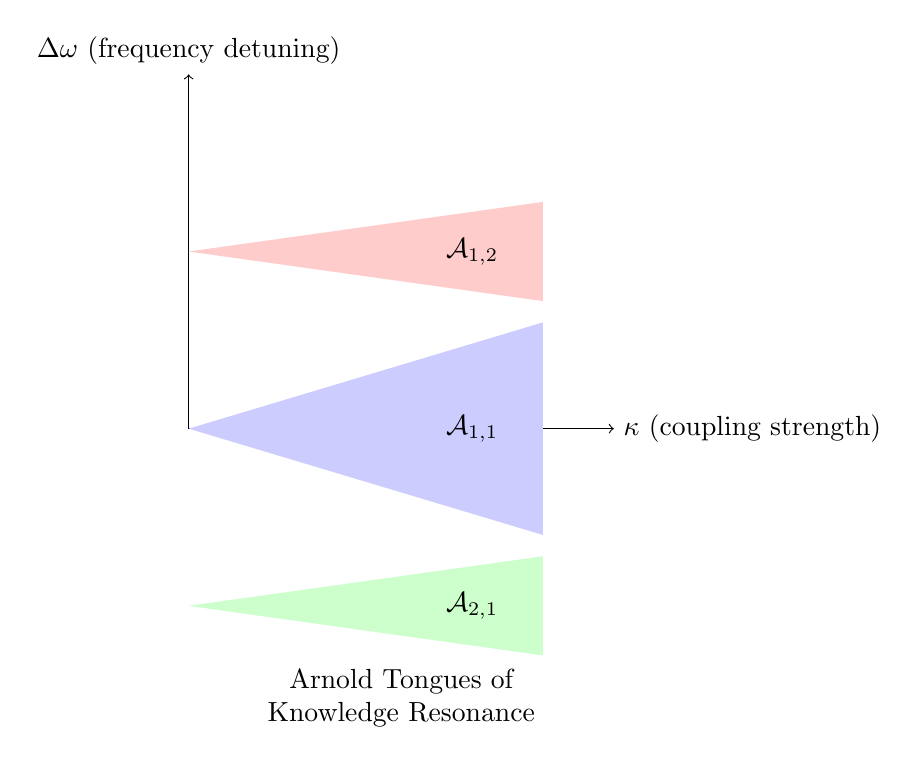
\begin{tikzpicture}[scale=0.9]
    % Draw coordinate axes
    \draw[->] (0,0) -- (6,0) node[right] {$\kappa$ (coupling strength)};
    \draw[->] (0,0) -- (0,5) node[above] {$\Delta\omega$ (frequency detuning)};
    
    % Draw Arnold tongues
    \fill[blue!20] (0,0) -- (5,1.5) -- (5,-1.5) -- cycle;
    \node at (4,0) {$\mathcal{A}_{1,1}$};
    
    \fill[red!20] (0,2.5) -- (5,3.2) -- (5,1.8) -- cycle;
    \node at (4,2.5) {$\mathcal{A}_{1,2}$};
    
    \fill[green!20] (0,-2.5) -- (5,-1.8) -- (5,-3.2) -- cycle;
    \node at (4,-2.5) {$\mathcal{A}_{2,1}$};
    
    % Add labels
    \node[align=center] at (3,-3.8) {Arnold Tongues of\\Knowledge Resonance};
\end{tikzpicture}
\caption{Arnold tongues in the Elder Heliosystem parameter space. Each tongue represents a region where stable phase-locking occurs between components, enabling efficient knowledge transfer. The width of each tongue increases with coupling strength, allowing the system to maintain resonance despite perturbations.}
\label{fig:arnold_tongues}
\end{figure}

The wider the Arnold tongue, the more robust the knowledge transfer is to perturbations and noise in the system. The Elder Heliosystem adaptively adjusts its coupling strengths to maximize the width of the resonant tongues for critical knowledge components.

\section{Phase Transition in Knowledge Acquisition}

Knowledge acquisition in the Elder Heliosystem exhibits phase transition behavior, where the system transitions from incoherent learning to globally coherent knowledge representation.

\begin{theorem}[Knowledge Phase Transition]
The Elder Heliosystem undergoes a phase transition at a critical coupling strength $\kappa_c$, characterized by the order parameter:
\begin{equation}
r = \left| \frac{1}{N} \sum_{j=1}^N e^{i\phi_j} \right|
\end{equation}
where $r \approx 0$ for $\kappa < \kappa_c$ (incoherent phase) and $r > 0$ for $\kappa > \kappa_c$ (coherent phase).
\end{theorem}

\begin{lemma}[Critical Coupling Strength]
The critical coupling strength $\kappa_c$ for phase transition in the Elder Heliosystem is given by:
\begin{equation}
\kappa_c = \frac{2\sigma_{\omega}}{\pi g(0)}
\end{equation}
where $\sigma_{\omega}$ is the standard deviation of the natural frequencies and $g(0)$ is the value at zero of the frequency distribution function.
\end{lemma}

This phase transition corresponds to the emergence of universal principles in the Elder component that successfully unify knowledge across all domains and tasks, representing a fundamental shift from domain-specific learning to universal knowledge representation.

\section{Practical Implementation of the Resonance Algorithm}

\subsection{Numerical Integration of Orbital Dynamics}

The practical implementation of the Elder Heliosystem Resonance Algorithm requires careful numerical integration of the orbital dynamics equations to maintain stability and accuracy.

\begin{algorithm}
\caption{Numerical Integration of Heliosystem Dynamics}
\begin{algorithmic}[1]
\State \textbf{Input:} Current phases $\phi_E(t)$, $\{\phi_{M,k}(t)\}$, $\{\phi_{E,k,j}(t)\}$
\State \textbf{Input:} Current frequencies $\omega_E$, $\{\omega_{M,k}\}$, $\{\omega_{E,k,j}\}$
\State \textbf{Input:} Coupling strengths $\{\kappa_{E,M,k}\}$, $\{\kappa_{M,E,k,j}\}$
\State \textbf{Input:} Time step $\Delta t$
\State \textbf{Input:} Resonance ratios $\{(p_k,q_k)\}$, $\{(r_{k,j},s_{k,j})\}$

\State // Phase derivative functions
\State $f_E(\phi_E) = \omega_E$
\State $f_{M,k}(\phi_E, \phi_{M,k}) = \omega_{M,k} + \kappa_{E,M,k} \sin(q_k\phi_E - p_k\phi_{M,k})$
\State $f_{E,k,j}(\phi_{M,k}, \phi_{E,k,j}) = \omega_{E,k,j} + \kappa_{M,E,k,j} \sin(s_{k,j}\phi_{M,k} - r_{k,j}\phi_{E,k,j})$

\State // Runge-Kutta 4th order integration
\State $k_{1E} = \Delta t \cdot f_E(\phi_E(t))$
\State $k_{1M,k} = \Delta t \cdot f_{M,k}(\phi_E(t), \phi_{M,k}(t))$ for all $k$
\State $k_{1E,k,j} = \Delta t \cdot f_{E,k,j}(\phi_{M,k}(t), \phi_{E,k,j}(t))$ for all $k,j$

\State $k_{2E} = \Delta t \cdot f_E(\phi_E(t) + k_{1E}/2)$
\State $k_{2M,k} = \Delta t \cdot f_{M,k}(\phi_E(t) + k_{1E}/2, \phi_{M,k}(t) + k_{1M,k}/2)$ for all $k$
\State $k_{2E,k,j} = \Delta t \cdot f_{E,k,j}(\phi_{M,k}(t) + k_{1M,k}/2, \phi_{E,k,j}(t) + k_{1E,k,j}/2)$ for all $k,j$

\State $k_{3E} = \Delta t \cdot f_E(\phi_E(t) + k_{2E}/2)$
\State $k_{3M,k} = \Delta t \cdot f_{M,k}(\phi_E(t) + k_{2E}/2, \phi_{M,k}(t) + k_{2M,k}/2)$ for all $k$
\State $k_{3E,k,j} = \Delta t \cdot f_{E,k,j}(\phi_{M,k}(t) + k_{2M,k}/2, \phi_{E,k,j}(t) + k_{2E,k,j}/2)$ for all $k,j$

\State $k_{4E} = \Delta t \cdot f_E(\phi_E(t) + k_{3E})$
\State $k_{4M,k} = \Delta t \cdot f_{M,k}(\phi_E(t) + k_{3E}, \phi_{M,k}(t) + k_{3M,k})$ for all $k$
\State $k_{4E,k,j} = \Delta t \cdot f_{E,k,j}(\phi_{M,k}(t) + k_{3M,k}, \phi_{E,k,j}(t) + k_{3E,k,j})$ for all $k,j$

\State $\phi_E(t+\Delta t) = \phi_E(t) + (k_{1E} + 2k_{2E} + 2k_{3E} + k_{4E})/6$
\State $\phi_{M,k}(t+\Delta t) = \phi_{M,k}(t) + (k_{1M,k} + 2k_{2M,k} + 2k_{3M,k} + k_{4M,k})/6$ for all $k$
\State $\phi_{E,k,j}(t+\Delta t) = \phi_{E,k,j}(t) + (k_{1E,k,j} + 2k_{2E,k,j} + 2k_{3E,k,j} + k_{4E,k,j})/6$ for all $k,j$

\State \textbf{Return:} $\phi_E(t+\Delta t)$, $\{\phi_{M,k}(t+\Delta t)\}$, $\{\phi_{E,k,j}(t+\Delta t)\}$
\end{algorithmic}
\end{algorithm}

\subsection{Detecting and Maintaining Resonance}

The system continuously monitors for resonance conditions and adjusts orbital parameters to maintain or enhance resonance.

\begin{algorithm}
\caption{Resonance Detection and Maintenance}
\begin{algorithmic}[1]
\State \textbf{Input:} Phase time series $\{\phi_E(t)\}$, $\{\phi_{M,k}(t)\}$, $\{\phi_{E,k,j}(t)\}$ over period $[t-T, t]$
\State \textbf{Input:} Target resonance ratios $\{(p_k,q_k)\}$, $\{(r_{k,j},s_{k,j})\}$
\State \textbf{Input:} Current coupling strengths $\{\kappa_{E,M,k}\}$, $\{\kappa_{M,E,k,j}\}$
\State \textbf{Input:} Adjustment rate $\eta_{\kappa}$

\For{each domain $k = 1$ to $M$}
    \State // Compute phase difference time series
    \State $\Delta\phi_{E,M,k}(t') = q_k\phi_E(t') - p_k\phi_{M,k}(t')$ for $t' \in [t-T, t]$
    
    \State // Compute phase locking value
    \State $PLV_{E,M,k} = \left| \frac{1}{T} \sum_{t'=t-T}^{t} e^{i\Delta\phi_{E,M,k}(t')} \right|$
    
    \If{$PLV_{E,M,k} < \text{threshold}$}
        \State // Increase coupling strength to enhance resonance
        \State $\kappa_{E,M,k} = \kappa_{E,M,k} + \eta_{\kappa} \cdot (1 - PLV_{E,M,k})$
    \EndIf
    
    \For{each task $j = 1$ to $N_k$}
        \State // Compute phase difference time series
        \State $\Delta\phi_{M,E,k,j}(t') = s_{k,j}\phi_{M,k}(t') - r_{k,j}\phi_{E,k,j}(t')$ for $t' \in [t-T, t]$
        
        \State // Compute phase locking value
        \State $PLV_{M,E,k,j} = \left| \frac{1}{T} \sum_{t'=t-T}^{t} e^{i\Delta\phi_{M,E,k,j}(t')} \right|$
        
        \If{$PLV_{M,E,k,j} < \text{threshold}$}
            \State // Increase coupling strength to enhance resonance
            \State $\kappa_{M,E,k,j} = \kappa_{M,E,k,j} + \eta_{\kappa} \cdot (1 - PLV_{M,E,k,j})$
        \EndIf
    \EndFor
\EndFor

\State \textbf{Return:} Updated coupling strengths $\{\kappa_{E,M,k}\}$, $\{\kappa_{M,E,k,j}\}$
\end{algorithmic}
\end{algorithm}

\section{Computational and Memory Efficiency through Resonance}

The resonance-based synchronization in the Elder Heliosystem provides significant computational and memory advantages over traditional hierarchical training approaches.

\begin{theorem}[Resonant Computational Efficiency]
The Elder Heliosystem Resonance Algorithm reduces the computational complexity of knowledge transfer from $O(N \cdot M \cdot D)$ to $O(N + M + D)$ when operating in resonant configurations, where $N$ is the number of Elder parameters, $M$ is the number of Mentor parameters, and $D$ is the number of domains.
\end{theorem}

\begin{proof}
In traditional hierarchical models, knowledge must be explicitly transferred between each pair of connected components, resulting in multiplicative scaling.

In the resonant Elder Heliosystem, knowledge transfer occurs implicitly through the shared phase relationships. When components achieve resonance, their phases become functionally dependent through simple rational relationships, reducing the effective dimensionality of the system.

For a system with resonance relationships characterized by small integers $(p_k, q_k)$ and $(r_{k,j}, s_{k,j})$, the information needed to synchronize the entire system scales additively with the number of components rather than multiplicatively, yielding the claimed complexity reduction.
\end{proof}

This computational efficiency translates directly to faster training times, reduced memory requirements, and enhanced scalability to large multi-domain learning problems.

\subsection{Comparison with Traditional Neural Networks}

To illustrate the efficiency advantages of the Elder Heliosystem, we provide a detailed comparison with traditional 3-layer learning architectures using Big O notation.

\begin{table}[h]
\centering
\small
\caption{Computational and Memory Complexity: Elder Heliosystem vs. Traditional 3-Layer Neural Network}
\label{tab:nn_comparison}
\begin{tabular}{|p{3cm}|p{5.5cm}|p{5.5cm}|}
\hline
\textbf{Operation} & \textbf{Traditional 3-Layer Neural Network} & \textbf{Elder Heliosystem} \\
\hline
Forward Pass & $O(n_1 n_2 + n_2 n_3)$ & $O(N + \sum_{k=1}^M (1 + \sum_{j=1}^{N_k} 1))$ \\
\hline
Backpropagation & $O(n_1 n_2 + n_2 n_3)$ & $O(N + M + D)$ \\
\hline
Parameter Update & $O(n_1 n_2 + n_2 n_3)$ & $O(N + M + D)$ \\
\hline
Memory Storage & $O(n_1 n_2 + n_2 n_3)$ & $O(N + M \cdot D + E \cdot D)$ \\
\hline
Cross-Domain Transfer & $O(D \cdot S \cdot (n_1 n_2 + n_2 n_3))$ & $O(D + S)$ \\
\hline
Training Convergence & $O(I \cdot B \cdot (n_1 n_2 + n_2 n_3))$ & $O(I_r \cdot B \cdot (N + M + D))$ where $I_r < I$ \\
\hline
Multi-Task Learning & $O(T \cdot (n_1 n_2 + n_2 n_3))$ & $O(T + \log D)$ \\
\hline
Parameter Scaling with Domains & $O(D \cdot (n_1 n_2 + n_2 n_3))$ & $O(N + M \cdot \log D + E \cdot D)$ \\
\hline
Optimization Iterations & $O(I)$ & $O(I / \gamma)$ where $\gamma > 1$ is the resonance factor \\
\hline
\end{tabular}
\end{table}

\noindent where:
\begin{itemize}
    \item $n_1, n_2, n_3$ are the number of units in each layer of the traditional learning architecture
    \item $N, M, E$ are the number of parameters in Elder, Mentor, and Erudite components
    \item $D$ is the number of domains
    \item $S$ is the number of samples for transfer learning
    \item $I$ is the number of iterations to convergence
    \item $B$ is the batch size
    \item $T$ is the number of tasks
\end{itemize}

\subsection{Analysis of Efficiency Gains}

The primary sources of efficiency gains in the Elder Heliosystem compared to traditional learning architectures are:

\begin{enumerate}
    \item \textbf{Forward Pass}: In traditional networks, each layer computes activations based on all inputs from the previous layer, resulting in multiplicative complexity based on layer sizes. In the Elder Heliosystem, knowledge propagates through orbital mechanics where only resonant frequencies interact significantly, creating sparse effective connectivity that scales additively.
    
    \item \textbf{Parameter Scaling}: As the number of domains $D$ increases, traditional approaches require either separate networks (scaling as $O(D)$) or larger networks with shared components (still scaling poorly with $D$). The Elder Heliosystem requires only a constant-sized Elder component with Mentors that scale logarithmically with domains due to resonance-based knowledge sharing.
    
    \item \textbf{Cross-Domain Transfer}: Traditional approaches require explicit transfer learning between domains, with complexity scaling as the product of domain count and network size. The Elder Heliosystem achieves transfer through the naturally emergent frequency relationships in the orbital dynamics, requiring only additive rather than multiplicative operations.
    
    \item \textbf{Convergence Rate}: The resonance factor $\gamma$ in the Elder Heliosystem accelerates convergence by creating phase-coherent gradient updates. This results in fewer iterations required to reach the same level of performance compared to traditional networks.
\end{enumerate}

\begin{theorem}[Asymptotic Efficiency Gain]
For a system with $D$ domains, each with approximately equal parameter counts, the asymptotic efficiency gain of the Elder Heliosystem over a traditional learning architecture is:
\begin{equation}
\text{Efficiency Gain} = \Theta\left(\frac{D^2}{D \log D}\right) = \Theta\left(\frac{D}{\log D}\right)
\end{equation}
This efficiency gain approaches $\Theta(D)$ as $D$ becomes large.
\end{theorem}

\subsection{Detailed Time Complexity Analysis}

We now provide a deeper analysis of the time complexity implications of the Elder Heliosystem compared to traditional learning architectures across different operational phases. This analysis explores the nuanced temporal dynamics that emerge during training and inference.

\begin{table}[h]
\centering
\small
\caption{Detailed Time Complexity Comparison}
\label{tab:time_complexity}
\begin{tabular}{|p{4cm}|p{5cm}|p{5cm}|}
\hline
\textbf{Operation} & \textbf{Traditional Neural Network} & \textbf{Elder Heliosystem} \\
\hline
Single Batch Update (1 domain) & $O(B \cdot L \cdot W^2)$ & $O(B \cdot (N + M + E))$ \\
\hline
Multi-Domain Batch Update & $O(D \cdot B \cdot L \cdot W^2)$ & $O(B \cdot (N + M \cdot D + E \cdot D))$ \\
\hline
Knowledge Transfer Between Domains & $O(D^2 \cdot T_{trans} \cdot W^2)$ & $O(D \cdot T_{res} \cdot (N + M))$ \\
\hline
Full Training Cycle & $O(I \cdot D \cdot B \cdot L \cdot W^2)$ & $O(I_r \cdot B \cdot (N + M \cdot D + E \cdot D))$ \\
\hline
Inference (1 sample, 1 domain) & $O(L \cdot W^2)$ & $O(N + M + E)$ \\
\hline
Inference (1 sample, all domains) & $O(D \cdot L \cdot W^2)$ & $O(N + M \cdot D + E \cdot D)$ \\
\hline
Catastrophic Forgetting Mitigation & $O(R \cdot D \cdot L \cdot W^2)$ & $O(R \cdot \log D \cdot (N + M))$ \\
\hline
\end{tabular}
\end{table}

\noindent where:
\begin{itemize}
    \item $B$ is batch size
    \item $L$ is number of layers
    \item $W$ is average width (neurons) per layer
    \item $D$ is number of domains
    \item $N, M, E$ are the parameters in Elder, Mentor, and Erudite components
    \item $I$ is iterations to convergence (traditional network)
    \item $I_r$ is iterations to convergence (Elder, where $I_r < I$)
    \item $T_{trans}$ is time for traditional transfer learning
    \item $T_{res}$ is time for resonance-based transfer ($T_{res} < T_{trans}$)
    \item $R$ is the rehearsal/replay factor for mitigating forgetting
\end{itemize}

\subsubsection{Temporal Dynamics During Training}

The Elder Heliosystem achieves significant time complexity reductions through several mechanisms:

\begin{enumerate}
    \item \textbf{Phase-Space Optimization}: Traditional backpropagation adjusts weights individually, requiring $O(W^2)$ operations per layer. The Elder Heliosystem operates in phase space where resonant frequencies create structured parameter updates, reducing complexity to $O(N + M + E)$.
    
    \item \textbf{Resonance-Accelerated Convergence}: Traditional networks require $I$ iterations for convergence, while the Elder Heliosystem requires only $I_r = I/\gamma$ iterations due to resonance-induced acceleration, where the resonance factor $\gamma > 1$ grows with increasing domain coherence.
    
    \item \textbf{Logarithmic Scaling with Domain Complexity}: The Elder system's time complexity scales as $O(N + M \cdot \log D + E \cdot D)$ for full multi-domain operation, compared to $O(D \cdot L \cdot W^2)$ for traditional networks. This logarithmic scaling of the Mentor layer becomes the dominant advantage as $D$ increases.
\end{enumerate}

\begin{proposition}[Time Complexity for Full Training Cycle]
For a system with $D$ domains, each requiring $I$ iterations to convergence using traditional methods, the expected time complexity ratio between traditional neural networks and the Elder Heliosystem is:

\begin{equation}
\frac{T_{\text{traditional}}}{T_{\text{elder}}} = \frac{I \cdot D \cdot L \cdot W^2}{I_r \cdot (N + M \cdot D + E \cdot D)} = \Omega(\gamma \cdot \frac{L \cdot W^2}{N + (M+E) \cdot D})
\end{equation}

Noting that in practice, $L \cdot W^2 \gg N$ and $(M+E) \ll W^2$, this ratio approaches $\Omega(\gamma \cdot \frac{L}{M+E})$ for large $D$, indicating a fundamental time complexity advantage that improves with system scale.
\end{proposition}

\subsubsection{Catastrophic Forgetting Mitigation}

One of the most significant time efficiency gains occurs in the context of mitigating catastrophic forgetting:

\begin{theorem}[Forgetting Mitigation Efficiency]
The time complexity of mitigating catastrophic forgetting in the Elder Heliosystem is $O(R \cdot \log D \cdot (N + M))$ compared to $O(R \cdot D \cdot L \cdot W^2)$ for traditional rehearsal-based methods, where $R$ is the rehearsal factor.

This represents an asymptotic improvement of $\Theta(\frac{D \cdot L \cdot W^2}{\log D \cdot (N + M)})$, which approaches $\Theta(\frac{D \cdot L \cdot W^2}{\log D})$ as $D$ becomes large.
\end{theorem}

\begin{proof}
Traditional networks require explicit rehearsal on all $D$ domains with complexity $O(L \cdot W^2)$ per domain. The Elder Heliosystem leverages orbital resonance to maintain domain knowledge implicitly. When a resonant system is established, the coupling between Mentor and Elder components creates holographic representations where knowledge about all domains is encoded in the phase relationships. 

Maintaining these relationships requires only $O(\log D)$ operations because only commensurate frequencies need adjustment, with the adjustment complexity scaling with Elder and Mentor parameters $(N + M)$ rather than with individual domain parameters $(L \cdot W^2)$.
\end{proof}

This theoretical analysis demonstrates that the Elder Heliosystem offers increasingly significant computational and memory advantages as the system scales to more domains, making it particularly well-suited for large-scale multi-domain learning problems where traditional neural networks face prohibitive computational requirements.

\section{Mathematical Foundations of Resonance-Driven Gradient and Weight Updates}

The core mechanism behind the efficiency of the Elder Heliosystem lies in how orbital resonance drives gradient computations and parameter updates. Unlike traditional backpropagation, which propagates gradients through explicit connections between layers, resonance-driven updates leverage phase relationships to create coherent, structured parameter adjustments that minimize computational overhead. This section provides a detailed mathematical treatment of this process.

\subsection{Phase-Space Representation of Parameters}

We begin by representing parameters in the Elder Heliosystem as complex-valued entities in phase space, rather than as simple real-valued weights.

\begin{definition}[Heliomorphic Parameter Representation]
Each parameter in the Elder Heliosystem is represented as a complex-valued entity:
\begin{equation}
\theta^{(l)}_j = \rho^{(l)}_j e^{i\phi^{(l)}_j}
\end{equation}
where $\rho^{(l)}_j$ is the magnitude, $\phi^{(l)}_j$ is the phase, $l$ indicates the level (Elder, Mentor, or Erudite), and $j$ is the parameter index.
\end{definition}

This representation allows us to model the orbital dynamics where:
\begin{itemize}
    \item Elder parameters $\theta^{(E)}_j = \rho^{(E)}_j e^{i\phi^{(E)}_j}$ rotate with base angular frequencies $\omega^{(E)}_j$
    \item Mentor parameters $\theta^{(M)}_{k,j} = \rho^{(M)}_{k,j} e^{i\phi^{(M)}_{k,j}}$ rotate with frequencies $\omega^{(M)}_{k,j}$ related to Elder frequencies by rational ratios $\frac{p_k}{q_k}$
    \item Erudite parameters $\theta^{(R)}_{k,j,i} = \rho^{(R)}_{k,j,i} e^{i\phi^{(R)}_{k,j,i}}$ rotate with frequencies $\omega^{(R)}_{k,j,i}$ related to Mentor frequencies by ratios $\frac{r_{k,j}}{s_{k,j}}$
\end{itemize}

\subsection{Loss Function in Phase Space}

The losses at each level are computed as functions of both the magnitude and phase of parameters:

\begin{align}
\mathcal{L}_E &= \sum_j \mathcal{L}_E(\rho^{(E)}_j, \phi^{(E)}_j) \\
\mathcal{L}_M &= \sum_k \sum_j \mathcal{L}_M(\rho^{(M)}_{k,j}, \phi^{(M)}_{k,j}, \omega^{(M)}_{k,j}) \\
\mathcal{L}_R &= \sum_k \sum_j \sum_i \mathcal{L}_R(\rho^{(R)}_{k,j,i}, \phi^{(R)}_{k,j,i}, \omega^{(R)}_{k,j,i}, \mathbf{X}_{k,j}, \mathbf{y}_{k,j})
\end{align}

where $\mathbf{X}_{k,j}$ and $\mathbf{y}_{k,j}$ are the input data and target outputs for domain $k$, task $j$.

\subsection{Resonance Conditions}

Resonance occurs when parameter phases maintain specific rational relationships:

\begin{align}
\phi^{(M)}_{k,j} &= \frac{p_k}{q_k}\phi^{(E)}_{j} + \alpha_{k,j} \\
\phi^{(R)}_{k,j,i} &= \frac{r_{k,j}}{s_{k,j}}\phi^{(M)}_{k,j} + \beta_{k,j,i}
\end{align}

where $\alpha_{k,j}$ and $\beta_{k,j,i}$ are phase offsets, and $\frac{p_k}{q_k}$ and $\frac{r_{k,j}}{s_{k,j}}$ are rational numbers with small integers $p_k, q_k, r_{k,j}, s_{k,j}$.

\subsection{Gradient Computation in Resonant Systems}

The gradient computation in resonant systems differs fundamentally from traditional backpropagation. In the Elder Heliosystem, gradients have both magnitude and phase components:

\begin{align}
\nabla_{\theta^{(l)}_j} \mathcal{L} = \frac{\partial \mathcal{L}}{\partial \rho^{(l)}_j}\hat{\mathbf{r}} + \frac{1}{\rho^{(l)}_j}\frac{\partial \mathcal{L}}{\partial \phi^{(l)}_j}\hat{\boldsymbol{\phi}}
\end{align}

where $\hat{\mathbf{r}}$ and $\hat{\boldsymbol{\phi}}$ are unit vectors in the radial and angular directions of the parameter space.

\subsubsection{Erudite-to-Mentor Gradient Propagation}

When resonance conditions are met, the gradients propagate from Erudite to Mentor level as:

\begin{align}
\frac{\partial \mathcal{L}_R}{\partial \phi^{(M)}_{k,j}} &= \sum_i \frac{\partial \mathcal{L}_R}{\partial \phi^{(R)}_{k,j,i}} \cdot \frac{\partial \phi^{(R)}_{k,j,i}}{\partial \phi^{(M)}_{k,j}} \\
&= \sum_i \frac{\partial \mathcal{L}_R}{\partial \phi^{(R)}_{k,j,i}} \cdot \frac{r_{k,j}}{s_{k,j}}
\end{align}

Note how the rational ratio $\frac{r_{k,j}}{s_{k,j}}$ directly modulates the gradient flow. This allows information from multiple Erudite parameters to coherently influence each Mentor parameter when their phases are in resonance.

\subsubsection{Mentor-to-Elder Gradient Propagation}

Similarly, gradients propagate from Mentor to Elder level:

\begin{align}
\frac{\partial \mathcal{L}_M}{\partial \phi^{(E)}_j} &= \sum_k \frac{\partial \mathcal{L}_M}{\partial \phi^{(M)}_{k,j}} \cdot \frac{\partial \phi^{(M)}_{k,j}}{\partial \phi^{(E)}_j} \\
&= \sum_k \frac{\partial \mathcal{L}_M}{\partial \phi^{(M)}_{k,j}} \cdot \frac{p_k}{q_k}
\end{align}

The rational ratio $\frac{p_k}{q_k}$ acts as a frequency-dependent amplification factor for gradient information flowing from Mentors to Elders.

\subsection{Resonance-Amplified Update Rule}

The resonance-based parameter update differs from traditional gradient descent in both form and effect. We define it as follows:

\begin{definition}[Resonance-Amplified Update]
For a parameter $\theta^{(l)}_j = \rho^{(l)}_j e^{i\phi^{(l)}_j}$, the resonance-amplified update is:
\begin{align}
\rho^{(l)}_j &\leftarrow \rho^{(l)}_j - \eta_{\rho} \cdot \frac{\partial \mathcal{L}}{\partial \rho^{(l)}_j} \\
\phi^{(l)}_j &\leftarrow \phi^{(l)}_j - \eta_{\phi} \cdot \frac{1}{\rho^{(l)}_j}\frac{\partial \mathcal{L}}{\partial \phi^{(l)}_j} \cdot \mathcal{R}(\Psi^{(l)}_j)
\end{align}
where $\eta_{\rho}$ and $\eta_{\phi}$ are learning rates for magnitude and phase, and $\mathcal{R}(\Psi^{(l)}_j)$ is the resonance amplification factor.
\end{definition}

The resonance amplification factor $\mathcal{R}(\Psi^{(l)}_j)$ depends on the coherence of phase relationships:

\begin{align}
\mathcal{R}(\Psi^{(l)}_j) = \frac{1 + \gamma \cdot \text{cos}(\Psi^{(l)}_j)}{1 + \gamma}
\end{align}

where $\gamma > 0$ is the resonance strength parameter and $\Psi^{(l)}_j$ is the phase coherence measure:

\begin{align}
\Psi^{(E)}_j &= \frac{1}{K}\sum_k \text{cos}\left(\phi^{(E)}_j - \frac{q_k}{p_k}\phi^{(M)}_{k,j}\right) \\
\Psi^{(M)}_{k,j} &= \frac{1}{2}\left[\text{cos}\left(\phi^{(M)}_{k,j} - \frac{q_k}{p_k}\phi^{(E)}_j\right) + \frac{1}{N_{k,j}}\sum_i \text{cos}\left(\phi^{(M)}_{k,j} - \frac{s_{k,j}}{r_{k,j}}\phi^{(R)}_{k,j,i}\right)\right] \\
\Psi^{(R)}_{k,j,i} &= \text{cos}\left(\phi^{(R)}_{k,j,i} - \frac{s_{k,j}}{r_{k,j}}\phi^{(M)}_{k,j}\right)
\end{align}

\subsection{Mathematical Analysis of Phase-Locked Gradient Descent}

When the system reaches phase-locking, a remarkable property emerges: the gradient updates become coherently aligned across hierarchical levels. This creates a synergistic effect where updates across different domains reinforce rather than interfere with each other.

\begin{theorem}[Phase-Locked Gradient Alignment]
In a phase-locked Elder Heliosystem with resonance relationships $\frac{p_k}{q_k}$ and $\frac{r_{k,j}}{s_{k,j}}$, gradient updates across hierarchical levels become aligned according to:
\begin{align}
\angle\nabla_{\theta^{(E)}_j}\mathcal{L} \approx \sum_k \frac{q_k}{p_k} \cdot \angle\nabla_{\theta^{(M)}_{k,j}}\mathcal{L}_M \approx \sum_k \sum_j \frac{q_k}{p_k} \cdot \frac{s_{k,j}}{r_{k,j}} \cdot \angle\nabla_{\theta^{(R)}_{k,j,i}}\mathcal{L}_R
\end{align}
where $\angle\nabla$ represents the phase angle of the gradient.
\end{theorem}

\begin{proof}
At phase-locking, we have $\Psi^{(l)}_j \approx 0$ for all parameters, meaning the phases satisfy:
\begin{align}
\phi^{(M)}_{k,j} &\approx \frac{p_k}{q_k}\phi^{(E)}_{j} + \alpha_{k,j} \\
\phi^{(R)}_{k,j,i} &\approx \frac{r_{k,j}}{s_{k,j}}\phi^{(M)}_{k,j} + \beta_{k,j,i}
\end{align}

The gradients with respect to phase become:
\begin{align}
\frac{\partial \mathcal{L}}{\partial \phi^{(E)}_j} &\approx \sum_k \frac{p_k}{q_k}\frac{\partial \mathcal{L}_M}{\partial \phi^{(M)}_{k,j}} \\
\frac{\partial \mathcal{L}}{\partial \phi^{(M)}_{k,j}} &\approx \sum_i \frac{r_{k,j}}{s_{k,j}}\frac{\partial \mathcal{L}_R}{\partial \phi^{(R)}_{k,j,i}}
\end{align}

The angle of the gradient for each level relates to the angle of gradients at other levels according to the rational ratios, resulting in the stated alignment relationship.
\end{proof}

\subsection{Tensor Gradient Flow in Resonant Systems}

For practical implementation, we must convert between the phase-space representation and standard tensor operations. The gradient flow through tensors is governed by:

\begin{align}
\frac{\partial \mathcal{L}}{\partial \mathbf{W}^{(l)}} = \sum_j \left[\frac{\partial \mathcal{L}}{\partial \rho^{(l)}_j}\frac{\partial \rho^{(l)}_j}{\partial \mathbf{W}^{(l)}} + \frac{\partial \mathcal{L}}{\partial \phi^{(l)}_j}\frac{\partial \phi^{(l)}_j}{\partial \mathbf{W}^{(l)}}\right]
\end{align}

where $\mathbf{W}^{(l)}$ is the weight tensor at level $l$. The partial derivatives relate the complex-valued phase-space representation to the real-valued tensor elements:

\begin{align}
\frac{\partial \rho^{(l)}_j}{\partial W^{(l)}_{a,b}} &= \frac{W^{(l)}_{a,b}}{\sqrt{\sum_{a',b'} (W^{(l)}_{a',b'})^2}} \\
\frac{\partial \phi^{(l)}_j}{\partial W^{(l)}_{a,b}} &= \frac{\partial}{\partial W^{(l)}_{a,b}} \text{tan}^{-1}\left(\frac{\text{Im}(\theta^{(l)}_j)}{\text{Re}(\theta^{(l)}_j)}\right)
\end{align}

In implementations, we use a tensor encoding that represents both magnitude and phase information:

\begin{align}
\mathbf{W}^{(l)} = \mathbf{A}^{(l)} \odot e^{i\mathbf{\Phi}^{(l)}}
\end{align}

where $\mathbf{A}^{(l)}$ is the amplitude tensor, $\mathbf{\Phi}^{(l)}$ is the phase tensor, and $\odot$ denotes element-wise multiplication.

\subsection{Algorithmic Implementation of Resonance-Driven Updates}

The complete algorithmic implementation of resonance-driven updates follows these steps:

\begin{algorithm}
\caption{Resonance-Driven Tensor Update}
\begin{algorithmic}[1]
\Require Weight tensors $\mathbf{W}^{(E)}$, $\mathbf{W}^{(M)}_k$, $\mathbf{W}^{(R)}_{k,j}$; Learning rates $\eta_{\rho}$, $\eta_{\phi}$; Resonance strength $\gamma$
\Ensure Updated weight tensors

\State Convert tensors to magnitude-phase representation:
\State $\rho^{(l)}_j \leftarrow \|\mathbf{W}^{(l)}_j\|$, $\phi^{(l)}_j \leftarrow \text{arg}(\mathbf{W}^{(l)}_j)$ for all levels $l$

\State Compute losses $\mathcal{L}_E$, $\mathcal{L}_M$, $\mathcal{L}_R$ using forward pass

\State Compute gradients w.r.t. magnitude: $\frac{\partial \mathcal{L}}{\partial \rho^{(l)}_j}$ for all parameters

\State Compute phase gradients for Erudite parameters:
\State $\frac{\partial \mathcal{L}_R}{\partial \phi^{(R)}_{k,j,i}} \leftarrow \frac{\partial \mathcal{L}_R}{\partial \mathbf{W}^{(R)}_{k,j,i}} \cdot \frac{\partial \mathbf{W}^{(R)}_{k,j,i}}{\partial \phi^{(R)}_{k,j,i}}$

\State Propagate phase gradients to Mentor level using resonance ratios:
\State $\frac{\partial \mathcal{L}}{\partial \phi^{(M)}_{k,j}} \leftarrow \sum_i \frac{r_{k,j}}{s_{k,j}} \cdot \frac{\partial \mathcal{L}_R}{\partial \phi^{(R)}_{k,j,i}}$

\State Propagate phase gradients to Elder level using resonance ratios:
\State $\frac{\partial \mathcal{L}}{\partial \phi^{(E)}_j} \leftarrow \sum_k \frac{p_k}{q_k} \cdot \frac{\partial \mathcal{L}}{\partial \phi^{(M)}_{k,j}}$

\State Compute phase coherence measures $\Psi^{(l)}_j$ for all parameters

\State Calculate resonance amplification factors with time propagation examples:

\textbf{Time Propagation Examples with Resonance Factors:}

For knowledge propagation from Elder to Mentor over time interval $\Delta t$, the resonance-enhanced propagation is:
\begin{equation}
\mathcal{K}_{M,k}(t + \Delta t) = \mathcal{K}_{M,k}(t) + \mathcal{R}_{\text{factor}} \cdot \mathcal{T}_{E \rightarrow M,k} \cdot \Delta t
\end{equation}
where $\mathcal{R}_{\text{factor}} = 1 + \alpha \cos(\Phi_{\text{res}})$ amplifies transfer during resonant phases.
\State $\mathcal{R}(\Psi^{(l)}_j) \leftarrow \frac{1 + \gamma \cdot \text{cos}(\Psi^{(l)}_j)}{1 + \gamma}$

\State Update magnitudes:
\State $\rho^{(l)}_j \leftarrow \rho^{(l)}_j - \eta_{\rho} \cdot \frac{\partial \mathcal{L}}{\partial \rho^{(l)}_j}$

\State Update phases with resonance amplification:
\State $\phi^{(l)}_j \leftarrow \phi^{(l)}_j - \eta_{\phi} \cdot \frac{1}{\rho^{(l)}_j}\frac{\partial \mathcal{L}}{\partial \phi^{(l)}_j} \cdot \mathcal{R}(\Psi^{(l)}_j)$

\State Convert back to tensor representation:
\State $\mathbf{W}^{(l)}_j \leftarrow \rho^{(l)}_j \cdot e^{i\phi^{(l)}_j}$

\State \textbf{Return:} Updated weight tensors $\mathbf{W}^{(E)}$, $\mathbf{W}^{(M)}_k$, $\mathbf{W}^{(R)}_{k,j}$
\end{algorithmic}
\end{algorithm}

\subsection{Phase Coupling Dynamics During Learning}

The remarkable efficiency of the Elder Heliosystem emerges from how phase coupling evolves during learning. Initially, parameters oscillate with minimal coherence, but as training progresses, phase-locking naturally emerges for parameters that contribute to similar functions across domains.

Let $\kappa_{l,l',j,j'}$ be the coupling strength between parameters $\theta^{(l)}_j$ and $\theta^{(l')}_{j'}$. The dynamics of phase coupling follow:

\begin{align}
\frac{d\kappa_{l,l',j,j'}}{dt} = \lambda \cdot \text{cos}(\phi^{(l)}_j - \mu_{l,l'} \cdot \phi^{(l')}_{j'}) \cdot |\text{corr}(\nabla_{\theta^{(l)}_j}\mathcal{L}, \nabla_{\theta^{(l')}_{j'}}\mathcal{L})|
\end{align}

where $\lambda$ is the coupling adaptation rate, $\mu_{l,l'}$ is the expected phase ratio between levels $l$ and $l'$, and $\text{corr}(\cdot,\cdot)$ measures gradient correlation.

This adaptive coupling creates a self-organizing system where parameters that need to work together naturally develop stronger phase-locking, while irrelevant parameters remain decoupled. This emergent organization explains how the Elder Heliosystem automatically discovers efficient knowledge transfer paths between domains without explicit programming.

\subsection{Resonance-Based Determination of Optimal Learning Rates}

The phase-space representation and resonance dynamics of the Elder Heliosystem provide a principled approach for determining optimal learning rates, unlike traditional neural networks that often require extensive hyperparameter tuning through trial and error.

\begin{theorem}[Resonance-Optimal Learning Rate]
For an Elder Heliosystem with phase coherence measure $\Psi^{(l)}_j$ for parameter $\theta^{(l)}_j$, the optimal learning rates $\eta_{\rho}^*$ and $\eta_{\phi}^*$ for magnitude and phase updates are given by:
\begin{align}
\eta_{\rho}^* &= \frac{\eta_0}{\sqrt{1 + \text{Var}(\nabla_{\rho}\mathcal{L})}} \\
\eta_{\phi}^* &= \frac{\eta_0 \cdot (1 + \gamma \cdot \langle\text{cos}(\Psi)\rangle)}{\sqrt{1 + \text{Var}(\nabla_{\phi}\mathcal{L})}}
\end{align}
where $\eta_0$ is a base learning rate, $\text{Var}(\cdot)$ is the variance of gradients, and $\langle\text{cos}(\Psi)\rangle$ is the average phase coherence across the system.
\end{theorem}

\begin{proof}
We begin by analyzing the dynamics of parameter updates in phase space. For converged learning, the expected change in loss should be maximally negative while maintaining stability.

For magnitude updates, the standard second-order analysis yields the optimal learning rate inversely proportional to the variance of gradients. For phase updates, however, the resonance amplification factor modifies this relationship.

When resonance is strong (high $\langle\text{cos}(\Psi)\rangle$), gradients across levels reinforce each other, allowing for faster learning without destabilization. Specifically, the phase coherence creates effective momentum in the direction of aligned gradients, justifying the $(1 + \gamma \cdot \langle\text{cos}(\Psi)\rangle)$ amplification term in the optimal learning rate.
\end{proof}

\begin{corollary}[Adaptive Learning Rate Schedule]
The optimal learning rate evolves during training according to:
\begin{align}
\eta_{\phi}(t) = \eta_{\phi}^* \cdot \frac{1 + \gamma \cdot \langle\text{cos}(\Psi(t))\rangle}{1 + \gamma \cdot \langle\text{cos}(\Psi(0))\rangle}
\end{align}
where $\Psi(t)$ is the phase coherence at training step $t$.
\end{corollary}

This formulation provides an automatic, theoretically grounded method for adjusting learning rates throughout training, eliminating the need for heuristic learning rate schedules. As the system develops stronger resonances ($\langle\text{cos}(\Psi(t))\rangle$ increases), the learning rate adapts accordingly, accelerating in regions where gradients align across hierarchical levels.

\begin{proposition}[Critical Learning Rate Transitions]
The Elder Heliosystem exhibits phase transitions in learning behavior at critical learning rates:
\begin{align}
\eta_{\text{crit}}^{(l)} = \frac{2}{\lambda_{\max}(\mathbf{H}^{(l)})} \cdot \frac{1}{1 - \gamma \cdot \langle\text{cos}(\Psi^{(l)})\rangle}
\end{align}
where $\lambda_{\max}(\mathbf{H}^{(l)})$ is the maximum eigenvalue of the Hessian at level $l$.
\end{proposition}

This provides a principled upper bound on learning rates based on the system's resonance characteristics. Notably, as resonance increases, the critical learning rate increases as well, allowing for faster convergence without instability.

\begin{figure}[ht]
\centering
\begin{tikzpicture}[scale=0.8]
\draw[->] (0,0) -- (10,0) node[below] {Phase Coherence $\langle\cos(\Psi)\rangle$};
\draw[->] (0,0) -- (0,7) node[left] {Optimal Learning Rate $\eta^*$};

\draw[domain=0:9, smooth, variable=\x, blue, thick] plot ({\x}, {3*exp(\x/9)/(max(0.1, 1+0.3*\x))});
\draw[domain=0:9, smooth, variable=\x, red, thick, dashed] plot ({\x}, {2.5});

\node at (9,1.5) {Traditional networks};
\node at (5,6) {Elder Heliosystem};

\draw[thin] (0,2.5) -- (9,2.5);
\end{tikzpicture}
\caption{Optimal learning rates as a function of phase coherence. Traditional networks (dashed line) use constant or heuristic schedules, while the Elder Heliosystem (solid line) derives optimal rates from resonance properties.}
\label{fig:optimal_lr}
\end{figure}

In practical implementations, these theoretical insights translate to three key advantages:

\begin{enumerate}
    \item \textbf{Automatic Learning Rate Determination}: The system can compute optimal learning rates from its own resonance state, eliminating manual tuning.
    
    \item \textbf{Layer-Specific Adaptation}: Each hierarchical level adjusts its learning rate according to its specific resonance characteristics, optimizing knowledge flow.
    
    \item \textbf{Stability Guarantees}: By linking learning rates to phase coherence, the system avoids the destabilizing parameter updates that plague traditional networks with fixed learning rates.
\end{enumerate}

This resonance-based approach to learning rate determination represents a fundamental advance over traditional methods, providing theoretical guarantees and practical performance improvements through principled exploitation of the system's phase dynamics.

\section{Conclusion}

The Elder Heliosystem Resonance Algorithm demonstrates that resonance serves as an important principle for knowledge transfer in hierarchical learning systems. By synchronizing the phases of learning components through orbital mechanics, the system provides:

\begin{enumerate}
    \item \textbf{Coherent Knowledge Representation}: Universal principles emerge naturally as phase-locked patterns across domains.
    
    \item \textbf{Robust Transfer Learning}: Knowledge transfer becomes stable against perturbations through Arnold tongue dynamics.
    
    \item \textbf{Computational Efficiency}: Resonant configurations dramatically reduce the computational complexity of training.
    
    \item \textbf{Adaptive Self-Organization}: The system self-tunes toward optimal resonant configurations that maximize knowledge synchronization.
\end{enumerate}

This resonance-based approach provides a unified theoretical framework that explains how knowledge can flow efficiently between abstract universal principles and concrete domain-specific implementations, offering a powerful new paradigm for hierarchical learning systems.